\documentclass[tikz,border=8pt]{standalone}
\usepackage{tikz}
\usetikzlibrary{shapes,arrows,positioning}
\tikzstyle{proc}=[rectangle,draw,rounded corners,fill=blue!10,align=center,minimum width=3.4cm,minimum height=0.9cm,font=\small]
\tikzstyle{dec}=[diamond,draw,fill=green!10,align=center,aspect=2,font=\small]
\tikzstyle{term}=[rectangle,draw,rounded corners=8pt,fill=gray!15,align=center,minimum width=2.6cm,minimum height=0.9cm,font=\small\bfseries]
\tikzstyle{arr}=[->,thick]
\begin{document}
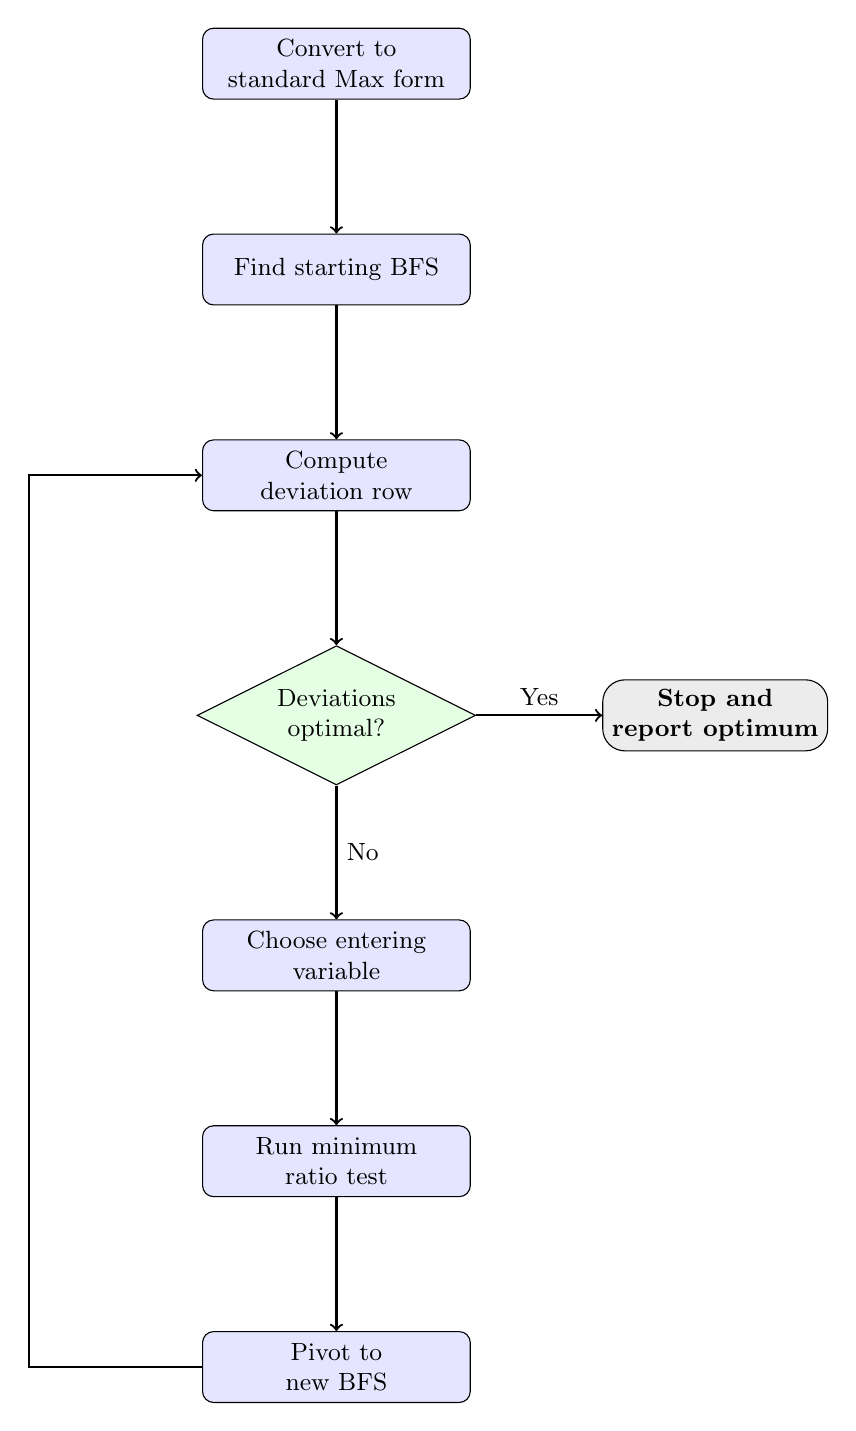
\begin{tikzpicture}[node distance=1.7cm]
\node[proc] (A) {Convert to\\standard Max form};
\node[proc, below=of A] (B) {Find starting BFS};
\node[proc, below=of B] (C) {Compute\\deviation row};
\node[dec, below=of C] (D) {Deviations\\optimal?};
\node[term, right=1.6cm of D] (E) {Stop and\\report optimum};
\node[proc, below=of D] (F) {Choose entering\\variable};
\node[proc, below=of F] (G) {Run minimum\\ratio test};
\node[proc, below=of G] (H) {Pivot to\\new BFS};
\draw[arr] (A) -- (B);
\draw[arr] (B) -- (C);
\draw[arr] (C) -- (D);
\draw[arr] (D) -- node[above, font=\small] {Yes} (E);
\draw[arr] (D) -- node[right, font=\small] {No} (F);
\draw[arr] (F) -- (G);
\draw[arr] (G) -- (H);
\draw[arr] (H.west) -- ++(-2.2cm,0) |- (C.west);
\end{tikzpicture}
\end{document}
